\begin{figure}[H]
  \centering
  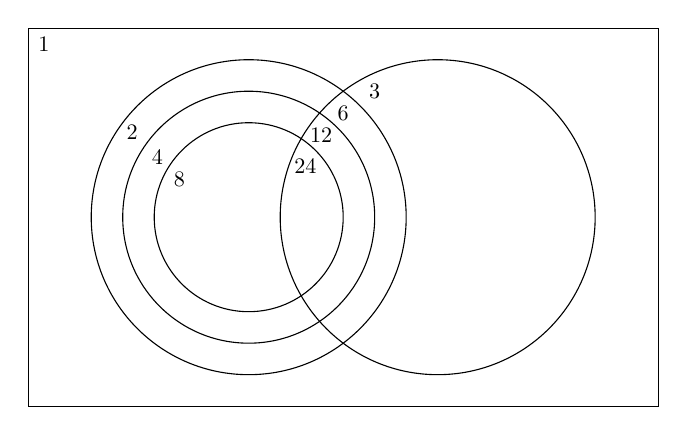
\begin{tikzpicture}[scale=0.8, every node/.style={scale=0.8}]
    \draw (0, 0) rectangle (10, 6);
    \draw (3.5, 3) circle (2.5);
    \draw (3.5, 3) circle (2);
    \draw (3.5, 3) circle (1.5);
    \draw (6.5, 3) circle (2.5);

    \node[] at (0.25, 5.75) {$1$};
    \node[] at (1.65, 4.35) {$2$};
    \node[] at (2.05, 3.95) {$4$};
    \node[] at (2.40, 3.60) {$8$};

    \node[] at (5.50, 5.00) {$3$};
    \node[] at (5.00, 4.65) {$6$};
    \node[] at (4.65, 4.30) {$12$};
    \node[] at (4.40, 3.80) {$24$};
  \end{tikzpicture}

  \caption{O colecție redundantă de mulțimi.}
  \label{fig:square-free-2}
\end{figure}
